\documentclass[a4paper,13pt]{article}

%%%%%%%%%%%%%%%%%%%%%%%%%%%%%%%%%%%%%%%%%%%%%%%%%%%%%%%%%%%%

% Global structure parameters
\usepackage{fullpage}%

\usepackage[francais]{babel}%

\usepackage[utf8]{inputenc}%
\usepackage[T1]{fontenc}%

\usepackage{mathpazo}%

% Macro packages
\usepackage{url}%
\usepackage{graphicx}%
\usepackage{minted}%
\usemintedstyle{borland}%

% for algorithm
\usepackage[french, onelanguage]{algorithm2e}
\usepackage{algorithmic}
% for tree
\usepackage{tikz}

%for floaw chart
\usetikzlibrary{arrows.meta}
\tikzset{%
  >={Latex[width=2mm,length=2mm]},
  % Specifications for style of nodes:
            base/.style = {rectangle, rounded corners, draw=black,
                           minimum width=4cm, minimum height=1cm,
                           text centered, font=\sffamily},
  mainFile/.style = {base, fill=blue!30},
       subFile/.style = {base, fill=red!30},
    module/.style = {base, fill=green!30},
        % process/.style = {base, minimum width=2.5cm, fill=orange!15,font=\ttfamily},
}

\usepackage{ragged2e}



% Fine tuning
\setlength{\parskip}{0.2\baselineskip plus 0.2\baselineskip}%

%%%%%%%%%%%%%%%%%%%%%%%%%%%%%%%%%%%%%%%%%%%%%%%%%%%%%%%%%%%%

\begin{document}

\title{Rapport Projet 0: Tours d'Hanoï et Pavage de Penrose}

\author{Bailluet Nicolas, Rémi Piau}

%\date{11 septembre 2018}

\maketitle

\begin{abstract}
  Ceci est un résumé.
\end{abstract}

%%%%%%%%%%%%%%%%%%%%%%%%%%%%%%%%%%%%%%%%%%%%%%%%%%%%%%%%%

\section{Les tours de Hanoï}

Le wikilivre est votre meilleur ami!
\begin{center}
  \url{https://fr.wikibooks.org/wiki/LaTeX}
\end{center}

test

%%%%%%%%%%%%%%%%%%%%%%%%%%%%%%%%%%%%%%%%%%%%%%%%%%%%%%%%%

\section{Pavage de Penrose}

Nous nous interressons au pavage de penrose sur un example avec des triangles isocèles de rapport $\phi$ entre leurs côtés (avec $\phi = \frac{1 + \sqrt{5}}{2}$, le nombre d'or).

\subsection{Solution initiale}
\subsection{Algorithme: un pavage par découpage récursif}
L'algorithme proposé pour le pavage est un découpage récursif d'un triangle de départ en sous triangles (voir l'agorithme \ref{algo:penrose}). Le découpage diffère en fonction de la nature du triangle obtu ou aïgu (voir figure \ref{fig:decoupage1}).
En reprenant les notation de la figure \ref{fig:decoupage1}, on peu écrire les formules de découpage qui reviennent à calculer la position du point $D$ dans le cas obtu et des points $D$ et $E$ dans l'autre cas. On a (avec $O$ l'origine du repère i.e $(0,0)$):
\[ \vec{OD} = \vec{OA} + \frac{\vec{AB}}{\phi}\]
pour le triangle obtu, et
\[ \vec{OD} = \vec{OC} - \frac{\vec{AC}}{\phi}\]

\[ \vec{OE} = \vec{OB} + \frac{\vec{BC}}{\phi}\]
pour le triangle aïgu.
\subsection{Implémentation: un code modulaire}

L'implémentation du pavage à été divisée en plusieurs fichier (voir figure \ref{fig:filesrelation} pour les relation entres ces fichier, une flèche vers un fichier indique que celui-ci est utilisé celui d'où part cette flèche).



\subsubsection{Une interface de programmation pour les triangles: api\_triangle.cma}
Nous avons réalisé une interface de programmation \mintinline{text}{api_triange.cma}.

Cette interface [\ref{code:apitrianglemli}] expose plusieurs types abstraits:
\begin{itemize}
	\item les type d'angles, aîgus ou obtus \mintinline{ocaml}{d!!!},
	\item les points représentés par un couple de flottant i.e. \mintinline{ocaml}{poi!!!},
	\item les triangle \mintinline{ocaml}{type triangle = !!!}, repésentés par une liste de points et un type d'angle.
\end{itemize}
Ces types ne sont accessibles et manipulables \emph{uniquement} travers des fonctions exposées par l'interface comme la fonction \mintinline{ocaml}{is_acute !!!}. On notera l'implémentation d'opérateurs infixe comme \mintinline{ocaml}{--}(soustraction) ou \mintinline{ocaml}{//}(division par un scalaire) qui permettent de manipuler le type point de manière élégante et plus compréhensible.

\subsubsection{Fichier pour les fonction graphiques: trgraphics.ml}
Ce fichier contient les fonctions permettant de facilement afficher les différents éléments du pavage (lignes, triangles) ainsi que les outils nécessaires au controle clavier de l'interface.

\subsection{Améliorations}

\subsubsection{Dessin unique des lignes de séparations: penrose\_noDoubleLine.ml}
Notre première amélioration concerne les lignes de découpes entre les triangles, ces dernière sont dessinées deux fois dans la première implémentation, une fois avec chaque triangle lors de l'affichage en utilisant la fonction \mintinline{ocaml}{draw_triangle_with_line} du fichier \mintinline{text}{trgraphics.ml}. Dans cette implémentation les lignes sont dessinées au fur et à mesure à chaque génération. En reprenant les notations de la figure \ref{fig:decoupage1}, on trace les lignes $AB$, $AC$, $BC$ pour le triangle initial puis à chaque division il suffit de tracer $CD$ si le triangle est obtu ou $DE$, $DB$ sinon avant de passer à la génération $(n-1)$ et de dessiner enfin les triangles sans bordure à la génération $0$ avec \mintinline{ocaml}{draw_triangle}.

\subsubsection{Déplacement et gestion des générations au clavier: penrose\_anime.ml}

Nous avons aussi réaliser une version du programme qui est capable de réagir au entrées clavier et qui permet ainsi de se déplacer sur le pavage, de changer d'échelle ainsi que de génération. Pour ce faire nous utilisons une boucle infinie bloquée par une fonction qui attend les évènements clavier et les passe à la fonction chargée du traitement de ces derniers. Pour faciliter la communication entre les différentes fonctions et la gestion des données, nous avons créé un nouveau type: \mintinline{ocaml}{type environnement = { mutable table:triangle list; mutable scale:float; mutable offset: point}}. Ce type une fois instancier permet de garder dans une seule variable tout l'information utile à l'affichage, c'est à dire le décalage par rapport au centre (offset), le grossissement (scale) ainsi que la liste (table) de tout les triangles de la génération courante. Cette liste permet grace à une fonction adaptée de calculer la generation suivante à partir de celle enregistrée, sans avoir besoin de recalculer toutes les divisions précédentes ce qui permet un gain important en performance quand le nombre de divisions est important. De plus pour éviter les scintillement dûs au temps de nécessaire pour le calcul puis le dessin ce programme utilise la techinque du "double buffering" qui consite à dessiner dans une mémoire tampon puis à afficher celui-ci. Cette amélioration permet de mieux comprendre le processus de pavage car l'utilisateur peu se déplacer à son gré dans celui-ci.


\section{Ma conclusion}
 
Les tours de Hanoï et le pavage de Penrose sont deux problèmes qui possèdent un intérêt pédagogique de par leur simplicité d'implémentation ce qui en fait de bon exemples pour l'apprentissage de la récursivité et des domaines où cette technique montre toute sa force. Mais ces sujets bien que simples en apparence deviennent vite très complexes si on relache un tant soit peut leurs hypothèses de construction ce qui les rends intéressant pour la recherche.


\appendix
\section{Une annexe: Penrose}
\newpage
\begin{figure}
\begin{algorithm}[H]
  \SetKwInOut{Input}{Entrées}
  \caption{Penrose($n$, $t$)}
  \Input{$n$ : nombre de générations, \newline
  $t$ : triangle initial}
  \eIf{$n = 0$}{ dessiner $t$}
  { Découper $t$ et appliquer Penrose($n-1$,$t_i$) pour chaque sous triangle $t_i$.
   }
  \end{algorithm}
  \label{algo:penrose}
 \end{figure}
  
\begin{figure}
  \begin{center}
    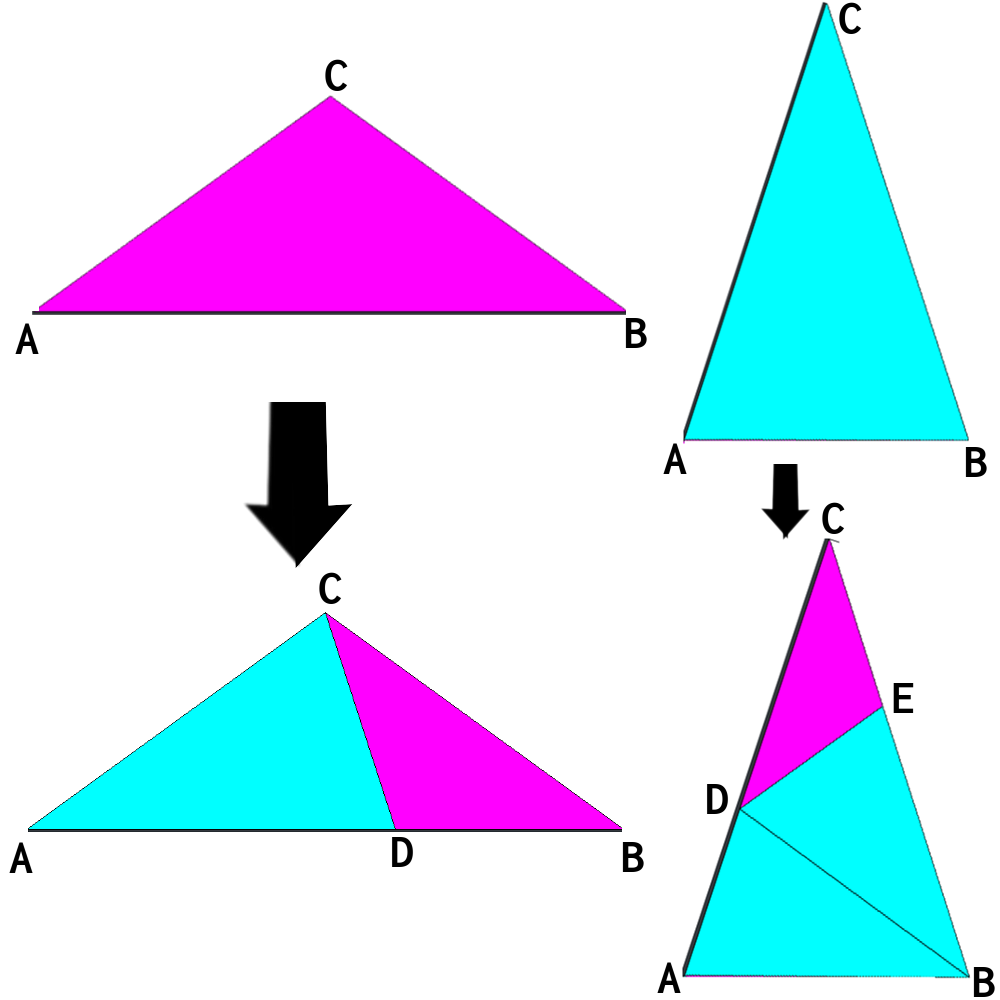
\includegraphics[width=12cm]{triangle-generation1.png}
    \caption{Division des triangles (obtus à gauche, aïgus à droite.}
    \label{fig:decoupage1}
  \end{center}
\end{figure}


\begin{figure}
\begin{center}
\begin{tikzpicture}[node distance=1.5cm,
    every node/.style={fill=white, font=\sffamily}, align=center]
  % Specification of nodes (position, etc.)
  \node (penrosebase) at (0,0)           [mainFile]          {penrose\_base.ml};
  \node (trgraphics) at (-3,-2)     [subFile]        {trgraphics.ml};
  \node (apitriangle) at (3, -2)     [module] {api\_triangle.cma};   
  % Specification of lines between nodes specified above
  % with aditional nodes for description 
  \draw[->]             (penrosebase) -- (apitriangle);
  \draw[->]     (penrosebase) -- (trgraphics);
  \draw[->]      (trgraphics) -- (apitriangle);
\end{tikzpicture}
\caption{Relations entre les fichiers}.
\label{fig:filesrelation} 
\end{center}
\end{figure}

\begin{figure}
\inputminted[frame=lines,linenos]{ocaml}{../penrose/api_triangle.mli}
\caption{api\_triangle.mli}
    \label{code:apitrianglemli}
\end{figure}

\end{document}
